\documentclass[a4paper,12pt]{article}
\usepackage[utf8]{inputenc}
\usepackage[T1]{fontenc}
\usepackage[includeheadfoot,margin=2cm]{geometry}
\usepackage{times}
\usepackage{booktabs}
\usepackage[small,compact]{titlesec}
\usepackage{enumitem}
\usepackage{amsmath}
\usepackage{amsthm}
\usepackage{mathptmx}
\usepackage{tikz}
\usetikzlibrary{shapes,arrows,decorations.pathreplacing}
\usepackage{xifthen}
\frenchspacing
\setlist{nosep}
\renewcommand{\ttdefault}{cmtt}
\author{Thor Kristoffersen}
\date{\today}
\title{How to Build a Machine}
\newcommand{\num}[1]{\texttt{#1}}
\newcommand{\hex}[1]{\num{#1}_{\textup{\tiny 16}}}
\newcommand{\bin}[1]{\num{#1}_{\textup{\tiny 2}}}
\newcommand{\MEM}[1]{\ifthenelse{\equal{#1}{}}{M}{M[#1]}}
\newcommand{\PC}{P}
\newcommand{\SP}{S}
\newcommand{\TERM}{T}
\newcommand{\F}{\bin{0}}
\newcommand{\T}{\bin{1}}
\newcommand{\octno}[2]{#1.\mathrm{octet}[#2]}
\newcommand{\bitno}[2]{#1.\mathrm{bit}[#2]}
\newcommand{\range}[2]{\{#1,\ldots,#2\}}
\newcommand{\proc}[1]{\textsc{#1}}
\DeclareMathOperator{\MOD}{mod}
\newcommand{\modulo}[2]{#1 \MOD #2}
\newcommand{\comment}[1]{\begin{quote}[\textit{#1}]\end{quote}}
\newcommand{\deviceio}[1]{$\langle$#1$\rangle$}
\newcommand{\op}[1]{$#1$}
\theoremstyle{definition}
\newtheorem{definition}{Definition}
\newtheorem{test}{Test}
\newenvironment{memtable}{%
  \begin{trivlist}
    \item
    }{%
    \end{trivlist}}
\newenvironment{memcolumn}{%
  \begin{tabular}{@{}ll@{}}
%    $i$ & $\MEM{i}$ \\
    \hline}
    {%
    \hline
  \end{tabular}}
\newcommand{\memspace}{\qquad}
\newcommand{\EXIT}      [1]{\op{\hex{00}}}
\newcommand{\NOP}       [1]{\op{\hex{01}}}
\newcommand{\JUMP}      [1]{\op{\hex{02}}}
\newcommand{\JZFWD}     [1]{\op{\hex{03}}}
\newcommand{\JZBACK}    [1]{\op{\hex{04}}}
\newcommand{\SETSP}     [1]{\op{\hex{05}}}
\newcommand{\GETPC}     [1]{\op{\hex{06}}}
\newcommand{\GETSP}     [1]{\op{\hex{07}}}
\newcommand{\PUSHZ}     [1]{\op{\hex{08}}}
\newcommand{\PUSHB}     [1]{\op{\hex{09}}}
\newcommand{\PUSHS}     [1]{\op{\hex{0A}}}
\newcommand{\PUSHI}     [1]{\op{\hex{0B}}}
\newcommand{\PUSHL}     [1]{\op{\hex{0C}}}
\newcommand{\LOADB}     [1]{\op{\hex{10}}}
\newcommand{\LOADS}     [1]{\op{\hex{11}}}
\newcommand{\LOADI}     [1]{\op{\hex{12}}}
\newcommand{\LOADL}     [1]{\op{\hex{13}}}
\newcommand{\STOREB}    [1]{\op{\hex{14}}}
\newcommand{\STORES}    [1]{\op{\hex{15}}}
\newcommand{\STOREI}    [1]{\op{\hex{16}}}
\newcommand{\STOREL}    [1]{\op{\hex{17}}}
\newcommand{\ADD}       [1]{\op{\hex{20}}}
\newcommand{\MULT}      [1]{\op{\hex{21}}}
\newcommand{\DIV}       [1]{\op{\hex{22}}}
\newcommand{\REM}       [1]{\op{\hex{23}}}
\newcommand{\LT}        [1]{\op{\hex{24}}}
\newcommand{\AND}       [1]{\op{\hex{28}}}
\newcommand{\OR}        [1]{\op{\hex{29}}}
\newcommand{\NOT}       [1]{\op{\hex{2A}}}
\newcommand{\XOR}       [1]{\op{\hex{2B}}}
\newcommand{\POW}       [1]{\op{\hex{2C}}}
\newcommand{\PUTBYTE}   [1]{\op{\hex{F9}}}
\newcommand{\PUTCHAR}   [1]{\op{\hex{FA}}}
\newcommand{\ADDSAMPLE} [1]{\op{\hex{FB}}}
\newcommand{\SETPIXEL}  [1]{\op{\hex{FC}}}
\newcommand{\NEWFRAME}  [1]{\op{\hex{FD}}}
\newcommand{\READPIXEL} [1]{\op{\hex{FE}}}
\newcommand{\READFRAME} [1]{\op{\hex{FF}}}

\newlist{stepnumbers}{enumerate}{2}
\setlist[stepnumbers]{label=\textbf{\arabic*},labelsep=0.7em}
\newlist{stepletters}{enumerate}{1}
\setlist[stepletters]{label=\textbf{\alph*}}

\begin{document}

\maketitle

\noindent
This film contains programs and data.
The programs can be executed by a machine to convert the data into documents, pictures, sound, and moving pictures.
The purpose of this part of the film is to guide you through the process of building this machine.
To understand the guide, it is necessary to have knowledge of basic 20th-century mathematics and physics.

When you have finished the machine, you will need to install an initial program in it before you can use it to execute programs.
This initial program is supplied as part of the film.

You will start by building a very simple machine, and then you will extend this machine through several stages, so that by the end you will have a fully functional machine.
Only when you have obtained the correct test results for each stage should you proceed with the following stage.

Number systems used here include decimal (number base 10), binary (number base 2), and hexadecimal (number base 16).
All non-decimal numbers are explictly indicated by subscripts indicating the number base in decimal.
Further detail on binary and hexadecimal notation can be found in Section~\ref{sec:number-notation}.

\section{Memory}

To build the machine, you first need some form of memory to represent state consisting of binary digits (bits).

\subsection{Representing State}

An \emph{element} is a group of bits in the memory that forms a unit with respect to naming.
The number of bits in an element is called the \emph{size} of the element, and an element of size $n$ is called an $n$-bit element.
Each element has a unique name, so that it can be unambiguously referred to.
The following elements are employed by the machine:
\begin{itemize}
\item $\TERM$: This is a one 1-bit element.
\item $\PC$: This is a 64-bit element.
\item $\SP$: This is a 64-bit element.
\item $\MEM{i}$ for $i \in \range{A}{A+N-1}$: Each of these is an 8-bit element.
\end{itemize}
The collection of all $\MEM{i}$ elements is called $\MEM{}$.

$A$ is a constant so that $0 \le A < 2^{64}$, and it represents the start of $\MEM{}$.
$N$ is a constant so that $0 < N \le 2^{64}-A$, and it represents the number of elements in $\MEM{}$.
Both $A$ and $N$ must be known at the time the machine is started.
The minimum acceptable $N$ will be given as part of the documentation of the program to be executed.

A graphical depiction of the machine elements is shown in Section~\ref{sec:machine-elements}.

In addition to the elements defined in the list above, it will be necessary for some tasks to introduce \emph{temporary elements}.
The name and size of these temporary elements will be provided in each case, as explained in Section~\ref{sec:memory-operations}.

\subsection{Notation}

\begin{definition}
For any element, $x$, the notation $\bitno{x}{i}$ refers to bit $i$ in $x$. (The numbering of bits is defined in Section~\ref{sec:binary-notation}.)
\end{definition}

\begin{definition}
A group of 8 bits is called an \emph{octet}, and for any 64-bit element, $x$, the notation $\octno{x}{i}$ refers to octet $i$ in $x$, which is the octet consisting of the bits from $\bitno{x}{8i+7}$ to $\bitno{x}{8i}$.
\end{definition}

\begin{definition}
The elements $\MEM{i}$ are written as a table where the left column is $i$ and the right column is $\MEM{i}$.  For example,
\begin{memtable}
  \begin{memcolumn}
    $\hex{0}$ & $\hex{A0}$ \\
    $\hex{1}$ & $\hex{A1}$ \\
    $\hex{2}$ & $\hex{A2}$ \\
    $\hex{3}$ & $\hex{A3}$ \\
  \end{memcolumn}
\end{memtable}
so in this case $\MEM{\hex{2}} = \hex{A2}$.
\end{definition}

\begin{definition}
The modulo operation, $\modulo{x}{y}$, for $y>0$, is defined here as follows:
\[ \modulo{x}{y} = x - y \left \lfloor \frac{x}{y} \right \rfloor \]
where $\left \lfloor z \right \rfloor$ is defined as the unique integer such that $\left \lfloor z \right \rfloor \le z < (\left \lfloor z \right \rfloor + 1)$.
\end{definition}

\subsection{Basic Memory Operations}
\label{sec:memory-operations}

The following are basic memory operations that must be exist in your implementation.

\begin{definition}
``The value of an element, $x$'' means the contents as retrieved from $x$.
\end{definition}

\begin{definition}
``To set an element, $x$, to $v$'' means to store the value of $v$ in $x$.
\end{definition}

\begin{definition}
``The value of an octet, $\octno{x}{i}$'' means the contents as retrieved from that octet.
\end{definition}

\begin{definition}
``To set an octet, $\octno{x}{i}$, to $v$'' means to store the value of $v$ in that octet, while keeping all other contents of $x$ unchanged.
\end{definition}

\begin{definition}
``To initialize the temporary $n$-bit element, $x$, to $v$'' means to create a temporary element of size $n$, name it $x$, and store the value of $v$ in $x$.
\end{definition}

\begin{definition}
``To increment an element, $x$, by $n$'' means to set $v$ to the value of $x$ and then set $x$ to $\modulo{(v + n)}{2^s}$, where $s$ is the size of $x$.
\end{definition}

\begin{definition}
``To decrement an element, $x$, by $n$'' means to set $v$ to the value of $x$ and then set $x$ to $\modulo{(v - n)}{2^s}$, where $s$ is the size of $x$.
\end{definition}

\subsection{Testing the Memory Operations}

To test that the memory operations work as they should, do the following two tests 1000 times.

\begin{test}
  Verify that your operations for storing and getting the value of an element work for every element, $x$, of sizes 1, 8, and 64, including $\PC$, $\SP$, $\TERM$, and $\MEM{i}$, where $i \in \range{0}{2^8-1}$.
  \begin{stepnumbers}
  \item Initialize the temporary elements, $y$ and $z$, of size $s$.
  \item For all $i \in \range{0}{s-1}$, set $\bitno{y}{i}$ to a random bit value.
  \item For all $i \in \range{0}{s-1}$, set $\bitno{z}{i}$ to a random bit value.
  \item Set $x$ to $y$.
  \item Verify that $x = y$.
  \item Increment $x$ by $z$.
  \item Verify that $x = \modulo{(y + z)}{2^s}$.
  \item Decrement $x$ by $z$.
  \item Verify that $x = y$.
  \end{stepnumbers}
\end{test}

\begin{test}
  Verify that your octet operations work for every 64-bit element, $x$, and every octet, $\octno{x}{n}$ for all $n \in \range{0}{7}$.
  \begin{stepnumbers}
  \item Initialize the temporary element, $y$, of size 64.
  \item Initialize the temporary element, $z$, of size 8.
  \item For all $i \in \range{0}{s-1}$, set $\bitno{y}{i}$ to a random bit value.
  \item For all $i \in \range{0}{7}$, set $\bitno{z}{i}$ to a random bit value.
  \item Set $x$ to $y$.
  \item Set $\octno{x}{n}$ to $z$.
  \item Verify that $\octno{x}{n} = z$.
  \item Verify that $\octno{x}{i} = \octno{y}{i}$ where $i \in \range{0}{7}$ and $i \neq n$.
  \end{stepnumbers}
\end{test}

\subsection{Summary of Memory}

The entire state of the machine is contained in elements $\PC$, $\SP$, $\TERM$, $\MEM{i}$, and the constants $A$ and $N$.

\section{Basic Procedures}

You will need to implement five basic procedures that are frequently used by the machine.
These use the memory operations described in Section~\ref{sec:memory-operations}.

\subsection{\proc{Put} Octets}

Assume that we have two temporary 64-bit elements called $x$ and $a$, and that $n$ is either 1, 2, 4, or 8.
The expression ``\proc{Put} $n$ octets from $x$ into index $a$'' means to do the following steps:
\begin{stepnumbers}
\item Initialize the temporary 8-bit element $i$ to 0.
\item Do the following $n$ times:
  \begin{stepletters}
  \item Set $\MEM{a+i}$ to $\octno{x}{i}$.
  \item Increment $i$ by 1.
  \end{stepletters}
\end{stepnumbers}

\begin{test}
  To test \proc{Put}, do as follows, with $A=0$ and $N=16$:
  \begin{stepnumbers}
  \item Set $\MEM{i}$ to 0 for all $i \in \range{0}{2^4-1}$.
  \item Initialize the temporary 64-bit element $x$ to $\hex{A7A6A5A4A3A2A1A0}$.
  \item \proc{Put} 1 octet  from $x$ into index $\hex{01}$.
  \item \proc{Put} 2 octets from $x$ into index $\hex{02}$.
  \item \proc{Put} 4 octets from $x$ into index $\hex{04}$.
  \item \proc{Put} 8 octets from $x$ into index $\hex{08}$.
  \item Verify that the contents of the elements in $\MEM{}$ are as in the following table.
  \end{stepnumbers}

  \begin{memtable}
    \begin{memcolumn}
      $\hex{0}$ & $\hex{00}$ \\
      $\hex{1}$ & $\hex{A0}$ \\
      $\hex{2}$ & $\hex{A0}$ \\
      $\hex{3}$ & $\hex{A1}$ \\
    \end{memcolumn}
    \memspace
    \begin{memcolumn}
      $\hex{4}$ & $\hex{A0}$ \\
      $\hex{5}$ & $\hex{A1}$ \\
      $\hex{6}$ & $\hex{A2}$ \\
      $\hex{7}$ & $\hex{A3}$ \\
    \end{memcolumn}
    \memspace
    \begin{memcolumn}
      $\hex{8}$ & $\hex{A0}$ \\
      $\hex{9}$ & $\hex{A1}$ \\
      $\hex{A}$ & $\hex{A2}$ \\
      $\hex{B}$ & $\hex{A3}$ \\
    \end{memcolumn}
    \memspace
    \begin{memcolumn}
      $\hex{C}$ & $\hex{A4}$ \\
      $\hex{D}$ & $\hex{A5}$ \\
      $\hex{E}$ & $\hex{A6}$ \\
      $\hex{F}$ & $\hex{A7}$ \\
    \end{memcolumn}
  \end{memtable}
\end{test}

\subsection{\proc{Get} Octets}

Assume that we have a temporary 64-bit element called $a$ and that $n$ is either 1, 2, 4, or 8.
The expression ``\proc{Get} $n$ octets from index $a$ into $x$'' means to do the following steps:
\begin{stepnumbers}
\item Initialize the temporary 64-bit element $x$ to 0.
\item Initialize the temporary 8-bit element $i$ to 0.
\item Do the following $n$ times:
  \begin{stepletters}
  \item Set $\octno{x}{i}$ to $\MEM{a+i}$.
  \item Increment $i$ by 1.
  \end{stepletters}
\end{stepnumbers}
The temporary 64-bit element $x$ can now be used by other procedures.

\begin{test}
  To test \proc{Get}, first set $N=16$, and set the following elements of $\MEM{}$ to the provided values.
  \begin{memtable}
    \begin{memcolumn}
      $\hex{0}$ & $\hex{A0}$ \\
      $\hex{1}$ & $\hex{A1}$ \\
      $\hex{2}$ & $\hex{A2}$ \\
      $\hex{3}$ & $\hex{A3}$ \\
    \end{memcolumn}
    \memspace
    \begin{memcolumn}
      $\hex{4}$ & $\hex{A4}$ \\
      $\hex{5}$ & $\hex{A5}$ \\
      $\hex{6}$ & $\hex{A6}$ \\
      $\hex{7}$ & $\hex{A7}$ \\
    \end{memcolumn}
    \memspace
    \begin{memcolumn}
      $\hex{8}$ & $\hex{A8}$ \\
      $\hex{9}$ & $\hex{A9}$ \\
      $\hex{A}$ & $\hex{AA}$ \\
      $\hex{B}$ & $\hex{AB}$ \\
    \end{memcolumn}
    \memspace
    \begin{memcolumn}
      $\hex{C}$ & $\hex{AC}$ \\
      $\hex{D}$ & $\hex{AD}$ \\
      $\hex{E}$ & $\hex{AE}$ \\
      $\hex{F}$ & $\hex{AF}$ \\
    \end{memcolumn}
  \end{memtable}
  Then proceed as follows:
  \begin{stepnumbers}
  \item Initialize the temporary 64-bit element $x$ to $0$.
  \item \proc{Get} 1 octet  from index $\hex{01}$ into $x$.
  \item Verify that the value of $x$ is $\hex{00000000000000A1}$.
  \item \proc{Get} 2 octets from index $\hex{02}$ into $x$.
  \item Verify that the value of $x$ is $\hex{000000000000A3A2}$.
  \item \proc{Get} 4 octets from index $\hex{04}$ into $x$.
  \item Verify that the value of $x$ is $\hex{00000000A7A6A5A4}$.
  \item \proc{Get} 8 octets from index $\hex{08}$ into $x$.
  \item Verify that the value of $x$ is $\hex{AFAEADACABAAA9A8}$.
  \end{stepnumbers}
\end{test}
\subsection{\proc{Push} Element}

Assume that we have a temporary 64-bit element called $x$.
The expression ``\proc{Push} $x$'' means to do the following steps:
\begin{stepnumbers}
\item Decrement $\SP$ by 8.
\item \proc{Put} 8 octets from $x$ into index $\SP$.
\end{stepnumbers}

\begin{test}
  To test \proc{Push}, do as follows, with $N=16$:
  \begin{stepnumbers}
  \item Set $\MEM{i}$ to 0 for all $i \in \range{0}{2^N-1}$.
  \item Set $\SP$ to $\hex{10}$.
  \item Initialize the temporary 64-bit element $x$ to $\hex{AFAEADACABAAA9A8}$.
  \item Initialize the temporary 64-bit element $y$ to $\hex{A7A6A5A4A3A2A1A0}$.
  \item \proc{Push} $x$.
  \item Verify that the value of $\SP$ is $\hex{08}$.
  \item \proc{Push} $y$.
  \item Verify that the value of $\SP$ is $\hex{00}$.
  \item Verify that the contents of the elements in $\MEM{}$ are as in the following table.
  \end{stepnumbers}

  \begin{memtable}
    \begin{memcolumn}
      $\hex{0}$ & $\hex{A0}$ \\
      $\hex{1}$ & $\hex{A1}$ \\
      $\hex{2}$ & $\hex{A2}$ \\
      $\hex{3}$ & $\hex{A3}$ \\
    \end{memcolumn}
    \memspace
    \begin{memcolumn}
      $\hex{4}$ & $\hex{A4}$ \\
      $\hex{5}$ & $\hex{A5}$ \\
      $\hex{6}$ & $\hex{A6}$ \\
      $\hex{7}$ & $\hex{A7}$ \\
    \end{memcolumn}
    \memspace
    \begin{memcolumn}
      $\hex{8}$ & $\hex{A8}$ \\
      $\hex{9}$ & $\hex{A9}$ \\
      $\hex{A}$ & $\hex{AA}$ \\
      $\hex{B}$ & $\hex{AB}$ \\
    \end{memcolumn}
    \memspace
    \begin{memcolumn}
      $\hex{C}$ & $\hex{AC}$ \\
      $\hex{D}$ & $\hex{AD}$ \\
      $\hex{E}$ & $\hex{AE}$ \\
      $\hex{F}$ & $\hex{AF}$ \\
    \end{memcolumn}
  \end{memtable}
\end{test}

\subsection{\proc{Pop} Element}

The expression ``\proc{Pop} $x$'' means to do the following steps:
\begin{stepnumbers}
\item Initialize the temporary 64-bit element $x$ to 0.
\item \proc{Get} 8 octets from index $\SP$ into $x$.
\item Increment $\SP$ by 8.
\end{stepnumbers}
The 64-bit element $x$ can now be used by other procedures.

\begin{test}
  To test \proc{Pop}, first set $N=16$, set $S=0$, and set the following elements of $\MEM{}$ to the provided values.
  \begin{memtable}
    \begin{memcolumn}
      $\hex{0}$ & $\hex{A0}$ \\
      $\hex{1}$ & $\hex{A1}$ \\
      $\hex{2}$ & $\hex{A2}$ \\
      $\hex{3}$ & $\hex{A3}$ \\
    \end{memcolumn}
    \memspace
    \begin{memcolumn}
      $\hex{4}$ & $\hex{A4}$ \\
      $\hex{5}$ & $\hex{A5}$ \\
      $\hex{6}$ & $\hex{A6}$ \\
      $\hex{7}$ & $\hex{A7}$ \\
    \end{memcolumn}
    \memspace
    \begin{memcolumn}
      $\hex{8}$ & $\hex{A8}$ \\
      $\hex{9}$ & $\hex{A9}$ \\
      $\hex{A}$ & $\hex{AA}$ \\
      $\hex{B}$ & $\hex{AB}$ \\
    \end{memcolumn}
    \memspace
    \begin{memcolumn}
      $\hex{C}$ & $\hex{AC}$ \\
      $\hex{D}$ & $\hex{AD}$ \\
      $\hex{E}$ & $\hex{AE}$ \\
      $\hex{F}$ & $\hex{AF}$ \\
    \end{memcolumn}
  \end{memtable}
  Then proceed as follows:
  \begin{stepnumbers}
  \item Initialize the temporary 64-bit element $x$ to $0$.
  \item Initialize the temporary 64-bit element $y$ to $0$.
  \item \proc{Pop} $x$.
  \item Verify that $\SP = \hex{08}$ and that $x = \hex{A7A6A5A4A3A2A1A0}$.
  \item \proc{Pop} $y$.
  \item Verify that $\SP = \hex{10}$ and that $y = \hex{AFAEADACABAAA9A8}$.
  \end{stepnumbers}
\end{test}

\subsection{\proc{Fetch} Octets}

Assume that $n$ is either 1, 2, 4, or 8.
The expression ``\proc{Fetch} $n$ octets into $x$'' means to do the following steps:
\begin{stepnumbers}
\item Initialize the temporary 64-bit element $x$ to 0.
\item \proc{Get} $n$ octets from index $\PC$ into $x$.
\item Increment $\PC$ by $n$.
\end{stepnumbers}
The temporary 64-bit element $x$ can now be used by other procedures.

\begin{test}
  To test \proc{Fetch}, first set $N=16$, and set the following elements of $\MEM{}$ to the provided values.
  \begin{memtable}
    \begin{memcolumn}
      $\hex{0}$ & $\hex{A0}$ \\
      $\hex{1}$ & $\hex{A1}$ \\
      $\hex{2}$ & $\hex{A2}$ \\
      $\hex{3}$ & $\hex{A3}$ \\
    \end{memcolumn}
    \memspace
    \begin{memcolumn}
      $\hex{4}$ & $\hex{A4}$ \\
      $\hex{5}$ & $\hex{A5}$ \\
      $\hex{6}$ & $\hex{A6}$ \\
      $\hex{7}$ & $\hex{A7}$ \\
    \end{memcolumn}
    \memspace
    \begin{memcolumn}
      $\hex{8}$ & $\hex{A8}$ \\
      $\hex{9}$ & $\hex{A9}$ \\
      $\hex{A}$ & $\hex{AA}$ \\
      $\hex{B}$ & $\hex{AB}$ \\
    \end{memcolumn}
    \memspace
    \begin{memcolumn}
      $\hex{C}$ & $\hex{AC}$ \\
      $\hex{D}$ & $\hex{AD}$ \\
      $\hex{E}$ & $\hex{AE}$ \\
      $\hex{F}$ & $\hex{AF}$ \\
    \end{memcolumn}
  \end{memtable}
  Then proceed as follows:
  \begin{stepnumbers}
  \item Initialize the temporary 64-bit element $w$ to 0.
  \item \proc{Fetch} 1 octet into $w$.
  \item Verify that $\PC = \hex{01}$ and that $w = \hex{00000000000000A0}$.
  \item \proc{Fetch} 2 octets into $w$.
  \item Verify that $\PC = \hex{03}$ and that $w = \hex{000000000000A2A1}$.
  \item \proc{Fetch} 4 octets into $w$.
  \item Verify that $\PC = \hex{07}$ and that $w = \hex{00000000A6A5A4A3}$.
  \item \proc{Fetch} 8 octets into $w$.
  \item Verify that $\PC = \hex{0F}$ and that $w = \hex{AEADACABAAA9A8A7}$.
  \end{stepnumbers}
\end{test}

\subsection{Initialization of Memory}
\label{sec:initialization-of-memory}

Before the machine is started, the memory must be initialized.
With constants $A$ and $N$ known, the memory elements is initialized as follows.
\begin{itemize}
\item Set $\TERM$ to 0.
\item Set $\PC$ to $A$.
\item Set $\SP$ to $A+N$.
\item Store a program in $\MEM{}$.
  The program is a sequence of $n$ octets, and it is stored in $\MEM{i}$ for $i \in \range{A}{A+n-1}$.
\end{itemize}

\section{A Very Basic Machine}

You can now proceed with implementing a basic machine with $A=0$ and $N=265$.

Every time the machine starts, initialize the memory  as described in Section~\ref{sec:initialization-of-memory}.
Then execute the main procedure repeatedly until the value of $\TERM$ is $\T$.
The main procedure must carry out the following steps.
\begin{stepnumbers}
\item Initialize the temporary 64-bit element $k$ to 0.
\item \proc{Fetch} 1 octet into $k$.
\item\label{itm:main-case} If the value of $k$ is
  \begin{description}
  \item[\NOP{}] then do nothing.
  \item[\JUMP{}] then
    \begin{stepnumbers}
    \item Initialize the temporary 64-bit element $a$ to 0.
    \item \proc{Pop} $a$.
    \item Set $\PC$ to $a$.
    \end{stepnumbers}
  \item[\JZFWD{}] then
    \begin{stepnumbers}
    \item Initialize the temporary 64-bit elements $a$ and $x$ to 0.
    \item \proc{Fetch} 1 octet into $a$.
    \item \proc{Pop} $x$.
    \item If the value of $x$ is 0, then increment $\PC$ by $a$.
    \end{stepnumbers}
  \item[\JZBACK{}] then
    \begin{stepnumbers}
    \item Initialize the temporary 64-bit elements $a$ and $x$ to 0.
    \item \proc{Fetch} 1 octet into $a$.
    \item \proc{Pop} $x$.
    \item If the value of $x$ is 0, then decrement $\PC$ by $a + 1$.
    \end{stepnumbers}
  \item[\SETSP{}] then
    \begin{stepnumbers}
    \item Initialize the temporary 64-bit element $a$ to 0.
    \item \proc{Pop} $a$.
    \item Set $\SP$ to $a$.
    \end{stepnumbers}
  \item[\GETPC{}] then
    \begin{stepnumbers}
    \item Initialize the temporary 64-bit element $a$ to $\PC$.
    \item \proc{Push} $a$.
    \end{stepnumbers}
  \item[\GETSP{}] then
    \begin{stepnumbers}
    \item Initialize the temporary 64-bit element $a$ to $\SP$.
    \item \proc{Push} $a$.
    \end{stepnumbers}
  \item[\PUSHB{}] then
    \begin{stepnumbers}
    \item Initialize the temporary 64-bit element $a$ to 0.
    \item \proc{Fetch} 1 octet into $a$.
    \item \proc{Push} $a$.
    \end{stepnumbers}
  \end{description}
\item If the value of $k$ does not occur in the list in the previous point, then set $\TERM$ to $\T$.
\end{stepnumbers}

\begin{test}
  To test the machine, set the following elements of $\MEM{}$ to the provided values, set all other elements of $\MEM{}$ to 0, and start the machine.
  \begin{memtable}
    \begin{memcolumn}
      $\hex{00}$ & $\hex{01}$ \\
      $\hex{01}$ & $\hex{09}$ \\
      $\hex{02}$ & $\hex{1A}$ \\
      $\hex{03}$ & $\hex{09}$ \\
      $\hex{04}$ & $\hex{00}$ \\
      $\hex{05}$ & $\hex{09}$ \\
      $\hex{06}$ & $\hex{01}$ \\
      $\hex{07}$ & $\hex{09}$ \\
    \end{memcolumn}
    \memspace
    \begin{memcolumn}
      $\hex{08}$ & $\hex{15}$ \\
      $\hex{09}$ & $\hex{09}$ \\
      $\hex{0A}$ & $\hex{01}$ \\
      $\hex{0B}$ & $\hex{09}$ \\
      $\hex{0C}$ & $\hex{00}$ \\
      $\hex{0D}$ & $\hex{03}$ \\
      $\hex{0E}$ & $\hex{01}$ \\
      $\hex{0F}$ & $\hex{00}$ \\
    \end{memcolumn}
    \memspace
    \begin{memcolumn}
      $\hex{10}$ & $\hex{04}$ \\
      $\hex{11}$ & $\hex{02}$ \\
      $\hex{12}$ & $\hex{02}$ \\
      $\hex{13}$ & $\hex{00}$ \\
      $\hex{14}$ & $\hex{02}$ \\
      $\hex{15}$ & $\hex{03}$ \\
      $\hex{16}$ & $\hex{02}$ \\
      $\hex{17}$ & $\hex{04}$ \\
    \end{memcolumn}
    \memspace
    \begin{memcolumn}
      $\hex{18}$ & $\hex{04}$ \\
      $\hex{19}$ & $\hex{00}$ \\
      $\hex{1A}$ & $\hex{07}$ \\
      $\hex{1B}$ & $\hex{06}$ \\
      $\hex{1C}$ & $\hex{09}$ \\
      $\hex{1D}$ & $\hex{F8}$ \\
      $\hex{1E}$ & $\hex{05}$ \\
      $\hex{1F}$ & $\hex{00}$ \\
    \end{memcolumn}
  \end{memtable}
  When the machine terminates, the value of $\TERM$ should be $\T$, the value of $\PC$ should be $\hex{20}$, the value of $\SP$ should be $\hex{F8}$, and the following elements of $\MEM{}$ should have the indicated values.
  \begin{memtable}
    \begin{memcolumn}
      $\hex{E8}$ & $\hex{F8}$ \\
      $\hex{E9}$ & $\hex{00}$ \\
      $\hex{EA}$ & $\hex{00}$ \\
      $\hex{EB}$ & $\hex{00}$ \\
    \end{memcolumn}
    \memspace
    \begin{memcolumn}
      $\hex{EC}$ & $\hex{00}$ \\
      $\hex{ED}$ & $\hex{00}$ \\
      $\hex{EE}$ & $\hex{00}$ \\
      $\hex{EF}$ & $\hex{00}$ \\
    \end{memcolumn}
    \memspace
    \begin{memcolumn}
      $\hex{F0}$ & $\hex{1C}$ \\
      $\hex{F1}$ & $\hex{00}$ \\
      $\hex{F2}$ & $\hex{00}$ \\
      $\hex{F3}$ & $\hex{00}$ \\
    \end{memcolumn}
    \memspace
    \begin{memcolumn}
      $\hex{F4}$ & $\hex{00}$ \\
      $\hex{F5}$ & $\hex{00}$ \\
      $\hex{F6}$ & $\hex{00}$ \\
      $\hex{F7}$ & $\hex{00}$ \\
    \end{memcolumn}
    \memspace
    \begin{memcolumn}
      $\hex{F8}$ & $\hex{00}$ \\
      $\hex{F9}$ & $\hex{01}$ \\
      $\hex{FA}$ & $\hex{00}$ \\
      $\hex{FB}$ & $\hex{00}$ \\
    \end{memcolumn}
    \memspace
    \begin{memcolumn}
      $\hex{FC}$ & $\hex{00}$ \\
      $\hex{FD}$ & $\hex{00}$ \\
      $\hex{FE}$ & $\hex{00}$ \\
      $\hex{FF}$ & $\hex{00}$ \\
    \end{memcolumn}
  \end{memtable}
\end{test}

\section{Adding Bit-Copying Capabilities}

You can now add several more cases to step \ref{itm:main-case} of the main procedure.
These cases add bit-copying capabilities to the machine.

\begin{stepnumbers}[start=3]
\item If $k$ is
  \begin{description}
  \item[\LOADB{}] then
    \begin{stepnumbers}
    \item Initialize the temporary 64-bit elements $a$ and $x$ to 0.
    \item \proc{Pop} $a$.
    \item \proc{Get} 1 octet from index $a$ into $x$.
    \item \proc{Push} $x$.
    \end{stepnumbers}
  \item[\LOADS{}] then
    \begin{stepnumbers}
    \item Initialize the temporary 64-bit elements $a$ and $x$ to 0.
    \item \proc{Pop} $a$.
    \item \proc{Get} 2 octets from index $a$ into $x$.
    \item \proc{Push} $x$.
    \end{stepnumbers}
  \item[\LOADI{}] then
    \begin{stepnumbers}
    \item Initialize the temporary 64-bit elements $a$ and $x$ to 0.
    \item \proc{Pop} $a$.
    \item \proc{Get} 4 octets from index $a$ into $x$.
    \item \proc{Push} $x$.
    \end{stepnumbers}
  \item[\LOADL{}] then
    \begin{stepnumbers}
    \item Initialize the temporary 64-bit elements $a$ and $x$ to 0.
    \item \proc{Pop} $a$.
    \item \proc{Get} 8 octets from index $a$ into $x$.
    \item \proc{Push} $x$.
    \end{stepnumbers}
  \item[\STOREB{}] then
    \begin{stepnumbers}
    \item Initialize the temporary 64-bit elements $a$ and $x$ to 0.
    \item \proc{Pop} $a$.
    \item \proc{Pop} $x$.
    \item \proc{Put} 1 octet from $x$ into index $a$.
    \end{stepnumbers}
  \item[\STORES{}] then
    \begin{stepnumbers}
    \item Initialize the temporary 64-bit elements $a$ and $x$ to 0.
    \item \proc{Pop} $a$.
    \item \proc{Pop} $x$.
    \item \proc{Put} 2 octets from $x$ into index $a$.
    \end{stepnumbers}
  \item[\STOREI{}] then
    \begin{stepnumbers}
    \item Initialize the temporary 64-bit elements $a$ and $x$ to 0.
    \item \proc{Pop} $a$.
    \item \proc{Pop} $x$.
    \item \proc{Put} 4 octets from $x$ into index $a$.
    \end{stepnumbers}
  \item[\STOREL{}] then
    \begin{stepnumbers}
    \item Initialize the temporary 64-bit elements $a$ and $x$ to 0.
    \item \proc{Pop} $a$.
    \item \proc{Pop} $x$.
    \item \proc{Put} 8 octets from $x$ into index $a$.
    \end{stepnumbers}
  \end{description}
\end{stepnumbers}

\begin{test}
  To test the machine, set the following elements of $\MEM{}$ to the provided values, set all other elements of $\MEM{}$ to 0, and start the machine.
  \begin{memtable}
    \begin{memcolumn}
      $\hex{00}$ & $\hex{08}$ \\
      $\hex{01}$ & $\hex{19}$ \\
      $\hex{02}$ & $\hex{13}$ \\
      $\hex{03}$ & $\hex{08}$ \\
      $\hex{04}$ & $\hex{E0}$ \\
      $\hex{05}$ & $\hex{17}$ \\
      $\hex{06}$ & $\hex{08}$ \\
      $\hex{07}$ & $\hex{21}$ \\
    \end{memcolumn}
    \memspace
    \begin{memcolumn}
      $\hex{08}$ & $\hex{12}$ \\
      $\hex{09}$ & $\hex{08}$ \\
      $\hex{0A}$ & $\hex{E8}$ \\
      $\hex{0B}$ & $\hex{16}$ \\
      $\hex{0C}$ & $\hex{08}$ \\
      $\hex{0D}$ & $\hex{25}$ \\
      $\hex{0E}$ & $\hex{11}$ \\
      $\hex{0F}$ & $\hex{08}$ \\
    \end{memcolumn}
    \memspace
    \begin{memcolumn}
      $\hex{10}$ & $\hex{EC}$ \\
      $\hex{11}$ & $\hex{15}$ \\
      $\hex{12}$ & $\hex{08}$ \\
      $\hex{13}$ & $\hex{27}$ \\
      $\hex{14}$ & $\hex{10}$ \\
      $\hex{15}$ & $\hex{08}$ \\
      $\hex{16}$ & $\hex{EE}$ \\
      $\hex{17}$ & $\hex{14}$ \\
    \end{memcolumn}
    \memspace
    \begin{memcolumn}
      $\hex{18}$ & $\hex{00}$ \\
      $\hex{19}$ & $\hex{A0}$ \\
      $\hex{1A}$ & $\hex{A1}$ \\
      $\hex{1B}$ & $\hex{A2}$ \\
      $\hex{1C}$ & $\hex{A3}$ \\
      $\hex{1D}$ & $\hex{A4}$ \\
      $\hex{1E}$ & $\hex{A5}$ \\
      $\hex{1F}$ & $\hex{A6}$ \\
    \end{memcolumn}
    \memspace
    \begin{memcolumn}
      $\hex{20}$ & $\hex{A7}$ \\
      $\hex{21}$ & $\hex{A8}$ \\
      $\hex{22}$ & $\hex{A9}$ \\
      $\hex{23}$ & $\hex{AA}$ \\
      $\hex{24}$ & $\hex{AB}$ \\
      $\hex{25}$ & $\hex{AC}$ \\
      $\hex{26}$ & $\hex{AD}$ \\
      $\hex{27}$ & $\hex{AE}$ \\
    \end{memcolumn}
  \end{memtable}
  When the machine terminates, the value of $\SP$ should be $\hex{100}$, and the following elements of $\MEM{}$ should have the indicated values.
  \begin{memtable}
    \begin{memcolumn}
      $\hex{E0}$ & $\hex{A0}$ \\
      $\hex{E1}$ & $\hex{A1}$ \\
      $\hex{E2}$ & $\hex{A2}$ \\
      $\hex{E3}$ & $\hex{A3}$ \\
    \end{memcolumn}
    \memspace
    \begin{memcolumn}
      $\hex{E4}$ & $\hex{A4}$ \\
      $\hex{E5}$ & $\hex{A5}$ \\
      $\hex{E6}$ & $\hex{A6}$ \\
      $\hex{E7}$ & $\hex{A7}$ \\
    \end{memcolumn}
    \memspace
    \begin{memcolumn}
      $\hex{E8}$ & $\hex{A8}$ \\
      $\hex{E9}$ & $\hex{A9}$ \\
      $\hex{EA}$ & $\hex{AA}$ \\
      $\hex{EB}$ & $\hex{AB}$ \\
    \end{memcolumn}
    \memspace
    \begin{memcolumn}
      $\hex{EC}$ & $\hex{AC}$ \\
      $\hex{ED}$ & $\hex{AD}$ \\
      $\hex{EE}$ & $\hex{AE}$ \\
      $\hex{EF}$ & $\hex{00}$ \\
    \end{memcolumn}
  \end{memtable}
\end{test}

\section{Adding More Bit-Copying Capabilities}

You can now add several more cases to step \ref{itm:main-case} of the main procedure.
These cases add still more bit-copying capabilities to the machine.

\begin{stepnumbers}[start=3]
\item If $k$ is
  \begin{description}
  \item[\PUSHZ{}] then
    \begin{stepnumbers}
    \item Initialize the temporary 64-bit element $a$ to 0.
    \item \proc{Push} $a$.
    \end{stepnumbers}
  \item[\PUSHS{}] then
    \begin{stepnumbers}
    \item Initialize the temporary 64-bit element $a$ to 0.
    \item \proc{Fetch} 2 octets into $a$.
    \item \proc{Push} $a$.
    \end{stepnumbers}
  \item[\PUSHI{}] then
    \begin{stepnumbers}
    \item Initialize the temporary 64-bit element $a$ to 0.
    \item \proc{Fetch} 4 octets into $a$.
    \item \proc{Push} $a$.
    \end{stepnumbers}
  \item[\PUSHL{}] then
    \begin{stepnumbers}
    \item Initialize the temporary 64-bit element $a$ to 0.
    \item \proc{Fetch} 8 octets into $a$.
    \item \proc{Push} $a$.
    \end{stepnumbers}
  \end{description}
\end{stepnumbers}

\begin{test}
  To test the machine, set the following elements of $\MEM{}$ to the provided values, set all other elements of $\MEM{}$ to 0, and start the machine.
  \begin{memtable}
    \begin{memcolumn}
      $\hex{00}$ & $\hex{07}$ \\
      $\hex{01}$ & $\hex{09}$ \\
      $\hex{02}$ & $\hex{20}$ \\
      $\hex{03}$ & $\hex{21}$ \\
    \end{memcolumn}
    \memspace
    \begin{memcolumn}
      $\hex{04}$ & $\hex{0A}$ \\
      $\hex{05}$ & $\hex{10}$ \\
      $\hex{06}$ & $\hex{11}$ \\
      $\hex{07}$ & $\hex{12}$ \\
    \end{memcolumn}
    \memspace
    \begin{memcolumn}
      $\hex{08}$ & $\hex{13}$ \\
      $\hex{09}$ & $\hex{0B}$ \\
      $\hex{0A}$ & $\hex{00}$ \\
      $\hex{0B}$ & $\hex{01}$ \\
    \end{memcolumn}
    \memspace
    \begin{memcolumn}
      $\hex{0C}$ & $\hex{02}$ \\
      $\hex{0D}$ & $\hex{03}$ \\
      $\hex{0E}$ & $\hex{04}$ \\
      $\hex{0F}$ & $\hex{05}$ \\
    \end{memcolumn}
    \memspace
    \begin{memcolumn}
      $\hex{10}$ & $\hex{06}$ \\
      $\hex{11}$ & $\hex{07}$ \\
      $\hex{12}$ & $\hex{00}$ \\
      ~\\
    \end{memcolumn}
  \end{memtable}
  When the machine terminates, the value of $\SP$ should be $\hex{E0}$, and the following elements of $\MEM{}$ should have the indicated values.
  \begin{memtable}
    \begin{memcolumn}
      $\hex{E0}$ & $\hex{00}$ \\
      $\hex{E1}$ & $\hex{01}$ \\
      $\hex{E2}$ & $\hex{02}$ \\
      $\hex{E3}$ & $\hex{03}$ \\
      $\hex{E4}$ & $\hex{04}$ \\
      $\hex{E5}$ & $\hex{05}$ \\
      $\hex{E6}$ & $\hex{06}$ \\
      $\hex{E7}$ & $\hex{07}$ \\
    \end{memcolumn}
    \memspace
    \begin{memcolumn}
      $\hex{E8}$ & $\hex{10}$ \\
      $\hex{E9}$ & $\hex{11}$ \\
      $\hex{EA}$ & $\hex{12}$ \\
      $\hex{EB}$ & $\hex{13}$ \\
      $\hex{EC}$ & $\hex{00}$ \\
      $\hex{ED}$ & $\hex{00}$ \\
      $\hex{EE}$ & $\hex{00}$ \\
      $\hex{EF}$ & $\hex{00}$ \\
    \end{memcolumn}
    \memspace
    \begin{memcolumn}
      $\hex{F0}$ & $\hex{20}$ \\
      $\hex{F1}$ & $\hex{21}$ \\
      $\hex{F2}$ & $\hex{00}$ \\
      $\hex{F3}$ & $\hex{00}$ \\
      $\hex{F4}$ & $\hex{00}$ \\
      $\hex{F5}$ & $\hex{00}$ \\
      $\hex{F6}$ & $\hex{00}$ \\
      $\hex{F7}$ & $\hex{00}$ \\
    \end{memcolumn}
    \memspace
    \begin{memcolumn}
      $\hex{F8}$ & $\hex{00}$ \\
      $\hex{F9}$ & $\hex{00}$ \\
      $\hex{FA}$ & $\hex{00}$ \\
      $\hex{FB}$ & $\hex{00}$ \\
      $\hex{FC}$ & $\hex{00}$ \\
      $\hex{FD}$ & $\hex{00}$ \\
      $\hex{FE}$ & $\hex{00}$ \\
      $\hex{FF}$ & $\hex{00}$ \\
    \end{memcolumn}
  \end{memtable}
\end{test}

\section{Adding Arithmetic}

You can now add several more cases to step \ref{itm:main-case} of the main procedure.
These cases add arithmetic capabilities to the machine.

\begin{stepnumbers}[start=3]
\item If $k$ is
  \begin{description}
  \item[\ADD{}] then
    \begin{stepnumbers}
    \item Initialize the temporary 64-bit elements $x$ and $y$ to 0.
    \item \proc{Pop} $y$.
    \item \proc{Pop} $x$.
    \item \proc{Push} $\modulo{(x + y)}{2^{64}}$.
    \end{stepnumbers}
  \item[\MULT{}] then
    \begin{stepnumbers}
    \item Initialize the temporary 64-bit elements $x$ and $y$ to 0.
    \item \proc{Pop} $y$.
    \item \proc{Pop} $x$.
    \item \proc{Push} $\modulo{(x y)}{2^{64}}$.
    \end{stepnumbers}
  \item[\DIV{}] then
    \begin{stepnumbers}
    \item Initialize the temporary 64-bit elements $x$ and $y$ to 0.
    \item \proc{Pop} $y$.
    \item \proc{Pop} $x$.
    \item If $x > 0$ and $y > 0$,
      \begin{itemize}[label=]
      \item then \proc{Push} $q$, such that $x = qy + r$ and $0 \leq r < y$,
      \item otherwise \proc{Push} 0.
      \end{itemize}
    \end{stepnumbers}
  \item[\REM{}] then
    \begin{stepnumbers}
    \item Initialize the temporary 64-bit elements $x$ and $y$ to 0.
    \item \proc{Pop} $y$.
    \item \proc{Pop} $x$.
    \item If $x > 0$ and $y > 0$,
      \begin{itemize}[label=]
      \item then \proc{Push} $r$, such that $x = qy + r$ and $0 \leq r < y$,
      \item otherwise \proc{Push} 0.
      \end{itemize}
    \end{stepnumbers}
  \end{description}
\end{stepnumbers}
Note that in the preceding two cases, $q$ corresponds to the integer quotient, and $r$ corresponds to the integer remainder, of dividing $x$ by $y$.

\begin{test}
  To test the machine, set the following elements of $\MEM{}$ to the provided values, set all other elements of $\MEM{}$ to 0, and start the machine.
  \begin{memtable}
    \begin{memcolumn}
      $\hex{00}$ & $\hex{08}$ \\
      $\hex{01}$ & $\hex{1D}$ \\
      $\hex{02}$ & $\hex{13}$ \\
      $\hex{03}$ & $\hex{08}$ \\
      $\hex{04}$ & $\hex{25}$ \\
      $\hex{05}$ & $\hex{13}$ \\
      $\hex{06}$ & $\hex{20}$ \\
      $\hex{07}$ & $\hex{08}$ \\
    \end{memcolumn}
    \memspace
    \begin{memcolumn}
      $\hex{08}$ & $\hex{1D}$ \\
      $\hex{09}$ & $\hex{13}$ \\
      $\hex{0A}$ & $\hex{08}$ \\
      $\hex{0B}$ & $\hex{25}$ \\
      $\hex{0C}$ & $\hex{13}$ \\
      $\hex{0D}$ & $\hex{21}$ \\
      $\hex{0E}$ & $\hex{08}$ \\
      $\hex{0F}$ & $\hex{1D}$ \\
    \end{memcolumn}
    \memspace
    \begin{memcolumn}
      $\hex{10}$ & $\hex{13}$ \\
      $\hex{11}$ & $\hex{08}$ \\
      $\hex{12}$ & $\hex{25}$ \\
      $\hex{13}$ & $\hex{13}$ \\
      $\hex{14}$ & $\hex{22}$ \\
      $\hex{15}$ & $\hex{08}$ \\
      $\hex{16}$ & $\hex{1D}$ \\
      $\hex{17}$ & $\hex{13}$ \\
    \end{memcolumn}
    \memspace
    \begin{memcolumn}
      $\hex{18}$ & $\hex{08}$ \\
      $\hex{19}$ & $\hex{25}$ \\
      $\hex{1A}$ & $\hex{13}$ \\
      $\hex{1B}$ & $\hex{23}$ \\
      $\hex{1C}$ & $\hex{00}$ \\
      $\hex{1D}$ & $\hex{98}$ \\
      $\hex{1E}$ & $\hex{E7}$ \\
      $\hex{1F}$ & $\hex{D9}$ \\
    \end{memcolumn}
    \memspace
    \begin{memcolumn}
      $\hex{20}$ & $\hex{58}$ \\
      $\hex{21}$ & $\hex{1B}$ \\
      $\hex{22}$ & $\hex{C9}$ \\
      $\hex{23}$ & $\hex{77}$ \\
      $\hex{24}$ & $\hex{FF}$ \\
      $\hex{25}$ & $\hex{88}$ \\
      $\hex{26}$ & $\hex{60}$ \\
      $\hex{27}$ & $\hex{09}$ \\
    \end{memcolumn}
    \memspace
    \begin{memcolumn}
      $\hex{28}$ & $\hex{5C}$ \\
      $\hex{29}$ & $\hex{7D}$ \\
      $\hex{2A}$ & $\hex{2C}$ \\
      $\hex{2B}$ & $\hex{17}$ \\
      $\hex{2C}$ & $\hex{3F}$ \\
      \\
      \\
      \\
    \end{memcolumn}
  \end{memtable}
  When the machine terminates, the value of $\SP$ should be $\hex{E0}$, and the following elements of $\MEM{}$ should have the indicated values.
  \begin{memtable}
    \begin{memcolumn}
      $\hex{E0}$ & $\hex{78}$ \\
      $\hex{E1}$ & $\hex{65}$ \\
      $\hex{E2}$ & $\hex{B4}$ \\
      $\hex{E3}$ & $\hex{E8}$ \\
      $\hex{E4}$ & $\hex{25}$ \\
      $\hex{E5}$ & $\hex{17}$ \\
      $\hex{E6}$ & $\hex{1B}$ \\
      $\hex{E7}$ & $\hex{03}$ \\
    \end{memcolumn}
    \memspace
    \begin{memcolumn}
      $\hex{E8}$ & $\hex{04}$ \\
      $\hex{E9}$ & $\hex{00}$ \\
      $\hex{EA}$ & $\hex{00}$ \\
      $\hex{EB}$ & $\hex{00}$ \\
      $\hex{EC}$ & $\hex{00}$ \\
      $\hex{ED}$ & $\hex{00}$ \\
      $\hex{EE}$ & $\hex{00}$ \\
      $\hex{EF}$ & $\hex{00}$ \\
    \end{memcolumn}
    \memspace
    \begin{memcolumn}
      $\hex{F0}$ & $\hex{C0}$ \\
      $\hex{F1}$ & $\hex{08}$ \\
      $\hex{F2}$ & $\hex{F4}$ \\
      $\hex{F3}$ & $\hex{AE}$ \\
      $\hex{F4}$ & $\hex{F4}$ \\
      $\hex{F5}$ & $\hex{BB}$ \\
      $\hex{F6}$ & $\hex{CD}$ \\
      $\hex{F7}$ & $\hex{95}$ \\
    \end{memcolumn}
    \memspace
    \begin{memcolumn}
      $\hex{F8}$ & $\hex{20}$ \\
      $\hex{F9}$ & $\hex{48}$ \\
      $\hex{FA}$ & $\hex{E3}$ \\
      $\hex{FB}$ & $\hex{B4}$ \\
      $\hex{FC}$ & $\hex{98}$ \\
      $\hex{FD}$ & $\hex{F5}$ \\
      $\hex{FE}$ & $\hex{8E}$ \\
      $\hex{FF}$ & $\hex{3E}$ \\
    \end{memcolumn}
  \end{memtable}
\end{test}

\section{Adding More Arithmetic}

You can now add several more cases to step \ref{itm:main-case} of the main procedure.
These cases add more arithmetic capabilities to the machine.

\begin{stepnumbers}[start=3]
\item If $k$ is
  \begin{description}
  \item[\LT{}] then
    \begin{stepnumbers}
    \item Initialize the temporary 64-bit elements $x$ and $y$ to 0.
    \item \proc{Pop} $y$.
    \item \proc{Pop} $x$.
    \item If $x < y$,
      \begin{itemize}[label=]
      \item then \proc{Push} $2^{64} - 1$,
      \item otherwise \proc{Push} 0.
      \end{itemize}
    \end{stepnumbers}
  \item[\POW{}] then
    \begin{stepnumbers}
    \item Initialize the temporary 64-bit element $x$ to 0.
    \item \proc{Pop} $x$.
    \item If $x < 64$,
      \begin{itemize}[label=]
      \item then \proc{Push} $2^x$,
      \item otherwise \proc{Push} 0.
      \end{itemize}
    \end{stepnumbers}
  \end{description}
\end{stepnumbers}

\begin{test}
  To test the machine, set the following elements of $\MEM{}$ to the provided values, set all other elements of $\MEM{}$ to 0, and start the machine.
  \begin{memtable}
    \begin{memcolumn}
      $\hex{00}$ & $\hex{08}$ \\
      $\hex{01}$ & $\hex{24}$ \\
      $\hex{02}$ & $\hex{13}$ \\
      $\hex{03}$ & $\hex{08}$ \\
      $\hex{04}$ & $\hex{24}$ \\
      $\hex{05}$ & $\hex{13}$ \\
      $\hex{06}$ & $\hex{24}$ \\
      $\hex{07}$ & $\hex{08}$ \\
    \end{memcolumn}
    \memspace
    \begin{memcolumn}
      $\hex{08}$ & $\hex{24}$ \\
      $\hex{09}$ & $\hex{13}$ \\
      $\hex{0A}$ & $\hex{08}$ \\
      $\hex{0B}$ & $\hex{25}$ \\
      $\hex{0C}$ & $\hex{13}$ \\
      $\hex{0D}$ & $\hex{24}$ \\
      $\hex{0E}$ & $\hex{08}$ \\
      $\hex{0F}$ & $\hex{25}$ \\
    \end{memcolumn}
    \memspace
    \begin{memcolumn}
      $\hex{10}$ & $\hex{13}$ \\
      $\hex{11}$ & $\hex{08}$ \\
      $\hex{12}$ & $\hex{24}$ \\
      $\hex{13}$ & $\hex{13}$ \\
      $\hex{14}$ & $\hex{24}$ \\
      $\hex{15}$ & $\hex{08}$ \\
      $\hex{16}$ & $\hex{22}$ \\
      $\hex{17}$ & $\hex{10}$ \\
    \end{memcolumn}
    \memspace
    \begin{memcolumn}
      $\hex{18}$ & $\hex{2C}$ \\
      $\hex{19}$ & $\hex{08}$ \\
      $\hex{1A}$ & $\hex{23}$ \\
      $\hex{1B}$ & $\hex{10}$ \\
      $\hex{1C}$ & $\hex{2C}$ \\
      $\hex{1D}$ & $\hex{08}$ \\
      $\hex{1E}$ & $\hex{24}$ \\
      $\hex{1F}$ & $\hex{10}$ \\
    \end{memcolumn}
    \memspace
    \begin{memcolumn}
      $\hex{20}$ & $\hex{2C}$ \\
      $\hex{21}$ & $\hex{00}$ \\
      $\hex{22}$ & $\hex{40}$ \\
      $\hex{23}$ & $\hex{22}$ \\
      $\hex{24}$ & $\hex{00}$ \\
      $\hex{25}$ & $\hex{00}$ \\
      $\hex{26}$ & $\hex{00}$ \\
      $\hex{27}$ & $\hex{00}$ \\
    \end{memcolumn}
    \memspace
    \begin{memcolumn}
      $\hex{28}$ & $\hex{00}$ \\
      $\hex{29}$ & $\hex{00}$ \\
      $\hex{2A}$ & $\hex{00}$ \\
      $\hex{2B}$ & $\hex{00}$ \\
      $\hex{2C}$ & $\hex{A0}$ \\
      \\
      \\
      \\
    \end{memcolumn}
  \end{memtable}
  When the machine terminates, the value of $\SP$ should be $\hex{D0}$, and the following elements of $\MEM{}$ should have the indicated values.
  \begin{memtable}
    \begin{memcolumn}
      $\hex{D0}$ & $\hex{01}$ \\
      $\hex{D1}$ & $\hex{00}$ \\
      $\hex{D2}$ & $\hex{00}$ \\
      $\hex{D3}$ & $\hex{00}$ \\
      $\hex{D4}$ & $\hex{00}$ \\
      $\hex{D5}$ & $\hex{00}$ \\
      $\hex{D6}$ & $\hex{00}$ \\
      $\hex{D7}$ & $\hex{00}$ \\
    \end{memcolumn}
    \memspace
    \begin{memcolumn}
      $\hex{D8}$ & $\hex{00}$ \\
      $\hex{D9}$ & $\hex{00}$ \\
      $\hex{DA}$ & $\hex{00}$ \\
      $\hex{DB}$ & $\hex{00}$ \\
      $\hex{DC}$ & $\hex{04}$ \\
      $\hex{DD}$ & $\hex{00}$ \\
      $\hex{DE}$ & $\hex{00}$ \\
      $\hex{DF}$ & $\hex{00}$ \\
    \end{memcolumn}
    \memspace
    \begin{memcolumn}
      $\hex{E0}$ & $\hex{00}$ \\
      $\hex{E1}$ & $\hex{00}$ \\
      $\hex{E2}$ & $\hex{00}$ \\
      $\hex{E3}$ & $\hex{00}$ \\
      $\hex{E4}$ & $\hex{00}$ \\
      $\hex{E5}$ & $\hex{00}$ \\
      $\hex{E6}$ & $\hex{00}$ \\
      $\hex{E7}$ & $\hex{00}$ \\
    \end{memcolumn}
    \memspace
    \begin{memcolumn}
      $\hex{E8}$ & $\hex{00}$ \\
      $\hex{E9}$ & $\hex{00}$ \\
      $\hex{EA}$ & $\hex{00}$ \\
      $\hex{EB}$ & $\hex{00}$ \\
      $\hex{EC}$ & $\hex{00}$ \\
      $\hex{ED}$ & $\hex{00}$ \\
      $\hex{EE}$ & $\hex{00}$ \\
      $\hex{EF}$ & $\hex{00}$ \\
    \end{memcolumn}
    \memspace
    \begin{memcolumn}
      $\hex{F0}$ & $\hex{FF}$ \\
      $\hex{F1}$ & $\hex{FF}$ \\
      $\hex{F2}$ & $\hex{FF}$ \\
      $\hex{F3}$ & $\hex{FF}$ \\
      $\hex{F4}$ & $\hex{FF}$ \\
      $\hex{F5}$ & $\hex{FF}$ \\
      $\hex{F6}$ & $\hex{FF}$ \\
      $\hex{F7}$ & $\hex{FF}$ \\
    \end{memcolumn}
    \memspace
    \begin{memcolumn}
      $\hex{F8}$ & $\hex{00}$ \\
      $\hex{F9}$ & $\hex{00}$ \\
      $\hex{FA}$ & $\hex{00}$ \\
      $\hex{FB}$ & $\hex{00}$ \\
      $\hex{FC}$ & $\hex{00}$ \\
      $\hex{FD}$ & $\hex{00}$ \\
      $\hex{FE}$ & $\hex{00}$ \\
      $\hex{FF}$ & $\hex{00}$ \\
    \end{memcolumn}
  \end{memtable}
\end{test}

\section{Adding Bitwise Boolean Logic}

You can now add several more cases to step \ref{itm:main-case} of the main procedure.
These cases add bitwise Boolean logic capabilities to the machine.

\begin{stepnumbers}[start=3]
\item If $k$ is
  \begin{description}
  \item[\AND{}] then
    \begin{stepnumbers}
    \item Initialize the temporary 64-bit elements $x$, $y$, and $z$ to 0.
    \item \proc{Pop} $y$.
    \item \proc{Pop} $x$.
    \item For every $i \in \range{0}{63}$, if $\bitno{x}{i}$ is 1 and $\bitno{y}{i}$ is 1,
      \begin{itemize}[label=]
      \item then set $\bitno{z}{i}$ to 1,
      \item otherwise set $\bitno{z}{i}$ 0.
      \end{itemize}
    \item \proc{Push} $z$.
    \end{stepnumbers}
  \item[\OR{}] then
    \begin{stepnumbers}
    \item Initialize the temporary 64-bit elements $x$, $y$, and $z$ to 0.
    \item \proc{Pop} $y$.
    \item \proc{Pop} $x$.
    \item For every $i \in \range{0}{63}$, if $\bitno{x}{i}$ is 0 and $\bitno{y}{i}$ is 0,
      \begin{itemize}[label=]
      \item then set $\bitno{z}{i}$ to 0,
      \item otherwise set $\bitno{z}{i}$ to 1.
      \end{itemize}
    \item \proc{Push} $z$.
    \end{stepnumbers}
  \item[\NOT{}] then
    \begin{stepnumbers}
    \item Initialize the temporary 64-bit elements $x$ and $z$ to 0.
    \item \proc{Pop} $x$.
    \item For every $i \in \range{0}{63}$, if $\bitno{x}{i}$ is 1,
      \begin{itemize}[label=]
      \item then set $\bitno{z}{i}$ to 0,
      \item otherwise set $\bitno{z}{i}$ to 1.
      \end{itemize}
    \item \proc{Push} $z$.
    \end{stepnumbers}
  \item[\XOR{}] then
    \begin{stepnumbers}
    \item Initialize the temporary 64-bit elements $x$, $y$, and $z$ to 0.
    \item \proc{Pop} $y$.
    \item \proc{Pop} $x$.
    \item For every $i \in \range{0}{63}$, if $\bitno{x}{i}$ is different from $\bitno{y}{i}$,
      \begin{itemize}[label=]
      \item then set $\bitno{z}{i}$ to 1,
      \item otherwise set $\bitno{z}{i}$ to 0.
      \end{itemize}
    \item \proc{Push} the 64-bit value $z$.
    \end{stepnumbers}
  \end{description}
\end{stepnumbers}

\begin{test}
  To test the machine, set the following elements of $\MEM{}$ to the provided values, set all other elements of $\MEM{}$ to 0, and start the machine.
  \begin{memtable}
    \begin{memcolumn}
      $\hex{00}$ & $\hex{08}$ \\
      $\hex{01}$ & $\hex{1A}$ \\
      $\hex{02}$ & $\hex{13}$ \\
      $\hex{03}$ & $\hex{08}$ \\
      $\hex{04}$ & $\hex{22}$ \\
      $\hex{05}$ & $\hex{13}$ \\
      $\hex{06}$ & $\hex{28}$ \\
      $\hex{07}$ & $\hex{08}$ \\
    \end{memcolumn}
    \memspace
    \begin{memcolumn}
      $\hex{08}$ & $\hex{1A}$ \\
      $\hex{09}$ & $\hex{13}$ \\
      $\hex{0A}$ & $\hex{08}$ \\
      $\hex{0B}$ & $\hex{22}$ \\
      $\hex{0C}$ & $\hex{13}$ \\
      $\hex{0D}$ & $\hex{29}$ \\
      $\hex{0E}$ & $\hex{08}$ \\
      $\hex{0F}$ & $\hex{1A}$ \\
    \end{memcolumn}
    \memspace
    \begin{memcolumn}
      $\hex{10}$ & $\hex{13}$ \\
      $\hex{11}$ & $\hex{08}$ \\
      $\hex{12}$ & $\hex{22}$ \\
      $\hex{13}$ & $\hex{13}$ \\
      $\hex{14}$ & $\hex{2B}$ \\
      $\hex{15}$ & $\hex{08}$ \\
      $\hex{16}$ & $\hex{1A}$ \\
      $\hex{17}$ & $\hex{13}$ \\
    \end{memcolumn}
    \memspace
    \begin{memcolumn}
      $\hex{18}$ & $\hex{2A}$ \\
      $\hex{19}$ & $\hex{00}$ \\
      $\hex{1A}$ & $\hex{98}$ \\
      $\hex{1B}$ & $\hex{E7}$ \\
      $\hex{1C}$ & $\hex{D9}$ \\
      $\hex{1D}$ & $\hex{58}$ \\
      $\hex{1E}$ & $\hex{1B}$ \\
      $\hex{1F}$ & $\hex{C9}$ \\
    \end{memcolumn}
    \memspace
    \begin{memcolumn}
      $\hex{20}$ & $\hex{77}$ \\
      $\hex{21}$ & $\hex{FF}$ \\
      $\hex{22}$ & $\hex{88}$ \\
      $\hex{23}$ & $\hex{60}$ \\
      $\hex{24}$ & $\hex{09}$ \\
      $\hex{25}$ & $\hex{5C}$ \\
      $\hex{26}$ & $\hex{7D}$ \\
      $\hex{27}$ & $\hex{2C}$ \\
    \end{memcolumn}
    \memspace
    \begin{memcolumn}
      $\hex{28}$ & $\hex{17}$ \\
      $\hex{29}$ & $\hex{3F}$ \\
      \\
      \\
      \\
      \\
      \\
      \\
    \end{memcolumn}
  \end{memtable}
  When the machine terminates, the value of $\SP$ should be $\hex{E0}$, and the following elements of $\MEM{}$ should have the indicated values.
  \begin{memtable}
    \begin{memcolumn}
      $\hex{E0}$ & $\hex{67}$ \\
      $\hex{E1}$ & $\hex{18}$ \\
      $\hex{E2}$ & $\hex{26}$ \\
      $\hex{E3}$ & $\hex{A7}$ \\
      $\hex{E4}$ & $\hex{E4}$ \\
      $\hex{E5}$ & $\hex{36}$ \\
      $\hex{E6}$ & $\hex{88}$ \\
      $\hex{E7}$ & $\hex{00}$ \\
    \end{memcolumn}
    \memspace
    \begin{memcolumn}
      $\hex{E8}$ & $\hex{10}$ \\
      $\hex{E9}$ & $\hex{87}$ \\
      $\hex{EA}$ & $\hex{D0}$ \\
      $\hex{EB}$ & $\hex{04}$ \\
      $\hex{EC}$ & $\hex{66}$ \\
      $\hex{ED}$ & $\hex{E5}$ \\
      $\hex{EE}$ & $\hex{60}$ \\
      $\hex{EF}$ & $\hex{C0}$ \\
    \end{memcolumn}
    \memspace
    \begin{memcolumn}
      $\hex{F0}$ & $\hex{98}$ \\
      $\hex{F1}$ & $\hex{E7}$ \\
      $\hex{F2}$ & $\hex{D9}$ \\
      $\hex{F3}$ & $\hex{5C}$ \\
      $\hex{F4}$ & $\hex{7F}$ \\
      $\hex{F5}$ & $\hex{ED}$ \\
      $\hex{F6}$ & $\hex{77}$ \\
      $\hex{F7}$ & $\hex{FF}$ \\
    \end{memcolumn}
    \memspace
    \begin{memcolumn}
      $\hex{F8}$ & $\hex{88}$ \\
      $\hex{F9}$ & $\hex{60}$ \\
      $\hex{FA}$ & $\hex{09}$ \\
      $\hex{FB}$ & $\hex{58}$ \\
      $\hex{FC}$ & $\hex{19}$ \\
      $\hex{FD}$ & $\hex{08}$ \\
      $\hex{FE}$ & $\hex{17}$ \\
      $\hex{FF}$ & $\hex{3F}$ \\
    \end{memcolumn}
  \end{memtable}
\end{test}

\section{Joining the Machine With the Devices}
\label{sec:building-devices}

At this point you should have a machine with fully functional computational capabilities.
What you need to do now is to join the machine with the devices that allow it to consume data from its environment and to produce data to its environment.
There are four devices:
\begin{itemize}
\item The \emph{Image Input} device allows the machine to consume images as a two-dimensional array of gray-scale values.
  This device is very important, because it is what enables the machine to load programs encoded as images on the film.
\item The \emph{Image Output} device allows the machine to produce color images.
  Moving images are supported by producing a time series of still images.
\item The \emph{Audio Output} device allows the machine to produce audio signals as a time series of amplitude values.
\item The \emph{Text Output} device allows the machine to produce text as a stream of characters.
\end{itemize}
The descriptions below will only explain the correspondence between machine events and external events.
It is up to you to make sure that the interpretation of external events is faithfully implemented.
As before, you will add more cases to the existing machine.
Wherever external interaction is required, this is written \deviceio{like this}.

\subsection{Image Input}

The \emph{Image Input} device allows the machine to consume an image as a two-dimensional array of points of light intensity values.
The following figure shows an example of such an array, consisting of 32 sampling points arranged in 8 columns and 4 rows.
\begin{center}
  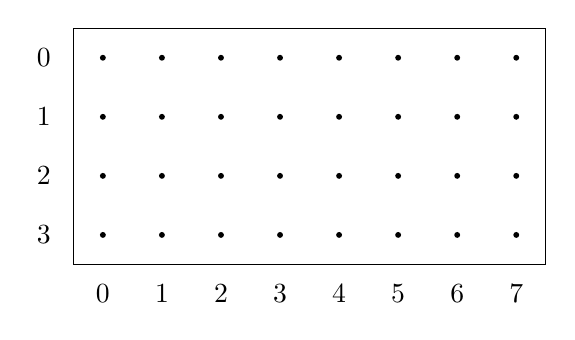
\begin{tikzpicture}[scale=0.75]
    \foreach \x in {0,...,7}
    \foreach \y in {0,...,3}
    {
      \fill (\x,\y) circle [radius=0.5mm,fill=black,draw] {};
    }
    \foreach \x in {0,...,7} \draw (\x, -1) node {\x};
    \foreach \y in {0,...,3} \draw (-1, 3 - \y) node {\y};
    \draw (-0.5,-0.5) -- (7.5,-0.5) -- (7.5,3.5) -- (-0.5,3.5) -- cycle;
  \end{tikzpicture}
\end{center}
As shown, both columns and rows are numbered consecutively, starting at 0.
The spacing between the sampling points must be uniform in both horizontal and vertical directions, and an anti-aliasing filter must be employed to limit the bandwidth of the image to satisfy the Nyquist-Shannon sampling theorem.

Each picture element detects the intensity of light transmitted or reflected at a sampling point in that particular position of the image, represented as one of 256 intensity levels, from 0 (minimum intensity) to 255 (maximum intensity).
Values between 0 and 255 represent intermediate intensities between these extremes.

In order to implement the image input device, you will need to add two extra cases to step \ref{itm:main-case} of the main procedure.

\begin{stepnumbers}[start=3]
\item If $k$ is
  \begin{description}
  \item[\READFRAME{}] then
    \begin{stepnumbers}
    \item Initialize the temporary 64-bit elements $c$ and $r$ to 0.
    \item \deviceio{Ready the next image to be consumed by the machine.}
    \item \deviceio{Find the number of columns and rows in the image.}
    \item Set $c$ to the number of columns in the image.
    \item \proc{Push} $c$.
    \item Set $r$ to the number of rows in the image.
    \item \proc{Push} $r$.
    \end{stepnumbers}
  \item[\READPIXEL{}] then
    \begin{stepnumbers}
    \item Initialize the temporary 64-bit elements $x$ and $y$ to 0.
    \item \proc{Pop} $x$.
    \item \proc{Pop} $y$.
    \item \deviceio{Measure the intensity of light at column $x$ and row $y$ in the image.}
    \item Set $z$ to the intensity level of light in the image at column $x$ and row $y$.
    \item \proc{Push} $z$.
    \end{stepnumbers}
  \end{description}
\end{stepnumbers}
In the last case, it is safe to assume that $0 \le x < c$ and $0 \le y < r$.

\subsection{Image Output}

The \emph{Image Output} device allows the machine to produce an image represented as a two-dimensional array of points of color space values.
Moving images can be produced as a sequence of images.

In order to implement the image output device, you will need to add two extra cases to step \ref{itm:main-case} of the main procedure.

\begin{stepnumbers}[start=3]
\item If $k$ is
  \begin{description}
  \item[\NEWFRAME{}] then
    \begin{stepnumbers}
    \item Finish and render the frame constructed so far.
    \item Initialize the temporary 64-bit elements $r$, $w$, and $h$ to 0.
    \item \proc{Pop} $r$.
    \item \proc{Pop} $h$.
    \item \proc{Pop} $w$.
    \item \deviceio{Set the audio sample rate to $r$, the width of the frame to $w$, and the height of the frame to $h$.}
    \end{stepnumbers}
  \item[\SETPIXEL{}] then
    \begin{stepnumbers}
    \item Initialize the temporary 64-bit elements  $x$, $y$, $r$, $g$, and $b$, to 0.
    \item \proc{Pop} $b$.
    \item \proc{Pop} $g$.
    \item \proc{Pop} $r$.
    \item \proc{Pop} $y$.
    \item \proc{Pop} $x$.
    \item \deviceio{Set the picture element at column $x$ and row $y$ to the point in the color space represented by the tuple $(r,g,b)$.}
    \end{stepnumbers}
  \end{description}
\end{stepnumbers}
In the last case, it is safe to assume that $0 \le x < w$ and $0 \le y < h$.
It is also safe to assume that all picture elements of a frame will have been set before it is finished and rendered.

When $\TERM{}$ is set to $\T$, the frame constructed so far must be rendered.

\subsection{Audio Output}

The \emph{Audio Output} device allows the machine to produce a two-channel audio signal encoded digitally using Linear Pulse Code Modulation.
The device must create an audio signal passing through a series of magnitude values specified by the program.
The bandwith of this audio signal must be less than half of the sampling frequency.
Each channel value is in the range $\range{0}{2^{16}-1}$.

In order to implement the audio output device, you will need to add one extra case to step \ref{itm:main-case} of the main procedure.

\begin{stepnumbers}[start=3]
\item If $k$ is
  \begin{description}
  \item[\ADDSAMPLE{}] then
    \begin{stepnumbers}
    \item Initialize the temporary 64-bit elements  $l$ and $r$ to 0.
    \item \proc{Pop} $r$.
    \item \proc{Pop} $l$.
    \item \deviceio{Set the audio signal magnitude of the left channel to $l$.}
    \item \deviceio{Set the audio signal magnitude of the right channel to $r$.}
    \end{stepnumbers}
  \end{description}
\end{stepnumbers}

\subsection{Text Output}

In order to implement the text output device, you will need to add one extra case to step \ref{itm:main-case} of the main procedure.

\begin{stepnumbers}[start=3]
  \setcounter{enumi}{2}
\item If $k$ is
  \begin{description}
  \item[\PUTCHAR{}] then
    \begin{stepnumbers}
    \item Initialize the temporary 64-bit element $c$ to 0.
    \item \proc{Pop} $c$.
    \item \deviceio{Produce the character with Unicode code point $c$.}
    \end{stepnumbers}
  \end{description}
\end{stepnumbers}

\subsection{Octet Output}

In order to implement the octet output device, you will need to add one extra case to step \ref{itm:main-case} of the main procedure.

\begin{stepnumbers}[start=3]
  \setcounter{enumi}{2}
\item If $k$ is
  \begin{description}
  \item[\PUTBYTE{}] then
    \begin{stepnumbers}
    \item Initialize the temporary 64-bit element $x$ to 0.
    \item Initialize the temporary 8-bit element $o$ to 0.
    \item \proc{Pop} $x$.
    \item For all $i \in \range{0}{7}$ set $\bitno{o}{i}$ to $\bitno{x}{i}$.
    \item \deviceio{Produce the number $o$.}
    \end{stepnumbers}
  \end{description}
\end{stepnumbers}

\section{Installing the Initial Program}

You first need to obtain the intial program from elsewhere on the film as a sequence of $p$ octets in hexadecimal notation.
These octets must be stored in $\MEM{i}$, where $i \in \range{A}{A+p-1}$.

The operation of the initial program, and programs loaded by the initial program, can be controlled by a set of parameters represented as a sequence of $q$ octets.
These octets must also be stored in $\MEM{}$.
This is done as follows:
\begin{stepnumbers}
  \item \proc{Put} 8 octets from $q$ into index $p$.
  \item Store the sequence of parameters in elements $\MEM{p+8}$ to $\MEM{p+8+q-1}$.
\end{stepnumbers}
When these things have been done, the machine can be started, and it can then load a program from the film and execute it.

\appendix

\section{Number Notation}
\label{sec:number-notation}

\subsection{Binary Notation}
\label{sec:binary-notation}

Each element contains a value represented as a sequence of binary digits.
In this documentation, individual binary digits are referred to using non-negative integers, listed in decreasing order.
For an $n$-bit value, the individual bits, $b_i$, are numbered as follows:
\[ b_{n-1} \; b_{n-2} \; \ldots \; b_{1} \; b_{0} \]
When an $n$-bit binary element is interpreted as a non-negative integer, the value of that integer is
\[
    v = \sum_{i=0}^{n-1} b_{i}2^{i}
\]

\subsection{Hexadecimal Notation}
\label{sec:hexadecimal-notation}

For convenience, binary numbers are normally written in hexadecimal notation.
Each hexadecimal digit corresponds to a group of four binary digits, as shown in the following table.

\begin{center}
  \begin{tabular}{@{}ll@{}}
    Hexadecimal digit & Binary digits \\
    \hline
    \num{0}           & \num{0000}   \\
    \num{1}           & \num{0001}   \\
    \num{2}           & \num{0010}   \\
    \num{3}           & \num{0011}   \\
    \num{4}           & \num{0100}   \\
    \num{5}           & \num{0101}   \\
    \num{6}           & \num{0110}   \\
    \num{7}           & \num{0111}   \\
    \hline
  \end{tabular}
  \hfil
  \begin{tabular}{@{}ll@{}}
    Hexadecimal digit & Binary digits \\
    \hline
    \num{8}           & \num{1000}   \\
    \num{9}           & \num{1001}   \\
    \num{A}           & \num{1010}   \\
    \num{B}           & \num{1011}   \\
    \num{C}           & \num{1100}   \\
    \num{D}           & \num{1101}   \\
    \num{E}           & \num{1110}   \\
    \num{F}           & \num{1111}   \\
    \hline
  \end{tabular}
\end{center}

\section{Machine Elements}
\label{sec:machine-elements}

The following is a graphical depiction of the machine elements.
\begin{trivlist}
\item 
  \centering\footnotesize
  \begin{tikzpicture}[scale=0.5]
    \foreach \y in {0,...,7}
    {
      \draw (0, 7-\y) node[anchor=east] {$\MEM{A+\y}$};
      \draw (0.5, \y) node[anchor=west,minimum width=16mm,minimum height=4mm,draw] {};
    }
    \draw (0, -1) node[anchor=east,minimum width=16mm] {$\vdots$};
    \draw (0.5, -1) node[anchor=west,minimum width=16mm] {$\vdots$};
    \draw (0, 11) node[anchor=east] {$\PC{}$};
    \draw (0, 9) node[anchor=east] {$\SP{}$};
    \draw (0, 13) node[anchor=east] {$\TERM{}$};
    \draw (0.5, 11) node[anchor=west,minimum width=128mm,minimum height=4mm,draw] {};
    \draw (0.5, 9) node[anchor=west,minimum width=128mm,minimum height=4mm,draw] {};
    \draw (0.5, 13) node[anchor=west,minimum width=2mm,minimum height=4mm,draw] {};
    \draw[decorate,decoration=brace] (5,7.5) -- (5,-1.5);
    \draw (6,3) node {$N$};
  \end{tikzpicture}
\end{trivlist}

\end{document}
